\documentclass[journal]{IEEEtran}
\usepackage{booktabs}
\usepackage{graphicx}
\usepackage{amsmath}
\usepackage{amssymb}
\usepackage{array}
\usepackage{url}
\usepackage{multirow}
\usepackage{xcolor}
\usepackage{microtype}

\title{Residual Coordination for Maritime Multi-UAV Search and Tracking\\
Under Sparse Communication}

\author{
\IEEEauthorblockN{Satish Kumar Mishra\textsuperscript{1}*,
Rashmi Gupta\textsuperscript{1}, and Ashfaq Khan\textsuperscript{1}}
\IEEEauthorblockA{\textsuperscript{1}Department of Electronics and Communication Engineering,\\
Netaji Subhas University of Technology, New Delhi 110078, India\\
*Corresponding author. Email: satishmishra135799@nsut.ac.in}
}

\begin{document}
\maketitle

% -----------------------------------------------------------------------
\begin{abstract}
We present a complete multi-UAV search-and-track system for maritime environments
where targets drift continuously and UAVs communicate only when their local belief
state changes significantly. Our central thesis is that sparse-reward multi-agent
problems require domain-structured priors: end-to-end learning cannot recover the
inductive bias provided by a well-designed base controller. The system is built in
three layers. First, a novel \emph{hybrid frontier-belief} base controller blends
lane-sweep coverage with occupancy-belief guidance under an event-triggered sparse
communication protocol. Second, a small two-layer MLP (25-16-2, tanh activations,
450 parameters) is trained via a custom evolutionary strategy (population 24, 100
iterations, 7 training seeds) to output bounded action corrections with scale
$\alpha = 0.25$---the \emph{fixed residual}. Third, we introduce two novel gating
mechanisms: a \emph{binary-gated} residual that suppresses corrections per UAV when
local belief confidence falls below a threshold, and a \emph{soft-gated} residual
that replaces the binary gate with a sigmoid for smooth, differentiable activation.

A pure MLP trained end-to-end with the same architecture achieves tracking ratios of
0.25--0.39 across scenarios, confirming that the structured base controller provides
essential inductive bias that end-to-end learning does not recover within the
evaluated compute budget. Evaluated over
30 fixed seeds per scenario across three difficulty levels (default, medium, hard),
the fixed residual reduces victim miss rate from 13.2\% to 11.8\% (default) and cuts
first-detection time from 3.37 to 2.37 steps (hard, $p < 0.001$). The soft-gated
variant achieves the best tracking on medium (0.913 vs.\ 0.879 hybrid, $p < 0.001$)
while the fixed residual dominates on first-detection speed. Compared against
Independent PPO (IPPO) with 20,165 parameters and a full learning rate sensitivity
study ($3\times10^{-4}$, $1\times10^{-4}$, $3\times10^{-5}$), our 450-parameter
residual achieves $1.65\times$ higher tracking ratio using $44.8\times$ fewer
parameters and fewer environment interactions---demonstrating that structured priors
dominate end-to-end RL on this class of problem. A robustness study under 0--60\%
packet drop rates shows all methods maintain performance within 0.001 tracking ratio,
demonstrating that event-triggered sparse communication provides inherent resilience
to communication failure. A sensor-noise study further confirms that all methods
maintain tracking above 0.894 under combined GPS noise (5\,m $\sigma$), probabilistic
detection decay, and 40\% actuation lag---without retraining. All code and trained
weights are publicly available.
\end{abstract}

% -----------------------------------------------------------------------
\section{Introduction}
\label{sec:intro}

Search and rescue at sea differs from land-based scenarios in one critical way:
targets do not stay put. Drifting victims, ocean currents, and limited UAV endurance
mean a swarm must continuously re-acquire targets rather than simply marking them
found. This makes the problem harder than standard coverage or exploration, because
the tracking component is ongoing rather than one-shot. A UAV that detects a victim
at step $t$ may lose contact by step $t{+}3$ if the victim has drifted outside the
sensing radius and no other UAV has taken over tracking.

The challenge is compounded by communication constraints. In maritime environments,
bandwidth is limited and radio links are unreliable. Continuous all-to-all
communication is impractical; UAVs must make decisions based primarily on local
observations, sharing information only when it is sufficiently novel to justify the
communication cost. This creates a fundamental tension: the UAVs need shared
situational awareness to coordinate tracking handoffs, but they cannot afford to
broadcast continuously.

\subsection{Prior Work}

Prior work on multi-robot exploration \cite{frontier_exploration} and decentralized
decision-making \cite{decentralized_pomdp} provides theoretical grounding, but most
assumes static targets or full communication. Coverage path planning surveys
\cite{coverage_path_planning} highlight lane-sweep and frontier methods as standard
baselines for area coverage, but these methods are designed for one-shot coverage
rather than persistent re-tracking. Maritime-specific work \cite{maritime_tracking,
uav_maritime_review, marine_multirobot_comm}
has started addressing drift and communication constraints, typically with centralized
planners that require continuous communication. Decentralized UAV swarms for SAR \cite{sar_swarms} have
shown promise without explicit communication, though persistent re-tracking after
initial discovery remains underexplored. Multi-agent trajectory planning for tracking
\cite{multi_robot_tracking} addresses coordination but not the search-then-track
transition under sparse communication.

Recent multi-UAV SAR work \cite{decentralized_uav_task, uav_sar_marl} has explored
reinforcement learning for task allocation, but relies on centralized training
infrastructure not available in our lightweight setting. End-to-end MARL methods such
as QMIX \cite{qmix} and MAPPO \cite{mappo} require centralized training and many
environment interactions; our evolutionary strategy \cite{es_openai} approach requires
neither, making it suitable for our lightweight simulator. Belief-based occupancy
tracking \cite{belief_propagation_tracking} underpins our grid update rule.

\subsection{Our Approach}

Our approach does not replace the handcrafted controller but corrects it. Residual
policy learning \cite{residual_rl, silver_residual, residual_rl_assembly} has worked well in manipulation, where a
model-based controller handles most of the task and a learned residual handles the
hard parts. We apply the same idea to maritime swarm coordination and introduce a
novel extension: a \emph{confidence-gated} residual that activates per UAV only when
its local belief confidence exceeds a threshold. This allows the residual to intervene
during tracking phases while leaving the base controller's sweep behavior intact
during search phases. The event-triggered communication scheme \cite{event_triggered,
sparse_comm_marl} is kept unchanged.

The key insight is that the base controller already handles the easy part of the
problem---systematic area coverage---very well. What it lacks is the ability to
fine-tune UAV positioning during the tracking phase, when a victim has been detected
and the UAV needs to stay close enough to maintain contact despite drift. The residual
MLP learns exactly this correction: given the current belief state, how should the
UAV deviate from its base trajectory to improve tracking?

We validate this thesis empirically by comparing against Independent PPO (IPPO)
\cite{mappo, ippo_reference}, a standard end-to-end MARL baseline with $44.8\times$ more parameters
(20,165 vs.\ 450) and more environment interactions. Despite a full learning rate
sensitivity study, IPPO's best result ($0.505$--$0.589$ tracking ratio) remains
$1.65\times$ below our method ($0.877$--$0.913$). This suggests that the performance
gap stems from the exploration challenge inherent to sparse-reward
maritime SAR rather than a tuning artifact.

\subsection{Contributions}

This paper makes the following contributions:
\begin{enumerate}
  \item A novel \emph{hybrid frontier-belief} base controller for maritime drifting-target
        SAR that combines lane-sweep coverage, frontier exploration, and belief-guided
        pursuit under event-triggered sparse communication.
  \item A \emph{fixed residual} policy trained via evolutionary strategy on top of the
        base controller, with a systematic evaluation over 30 seeds across three
        scenario difficulties.
  \item A \emph{binary-gated} residual variant that applies per-UAV state-dependent
        gating based on local belief confidence, preserving sweep behavior during
        low-information phases.
  \item A \emph{soft-gated} residual variant that replaces the binary gate with a
        sigmoid for smooth activation, achieving the best tracking on medium difficulty.
  \item An empirical demonstration that domain-structured priors outperform end-to-end
        MARL (IPPO) on sparse-reward maritime SAR: our 450-parameter residual achieves
        $1.65\times$ higher tracking ratio than a 20,165-parameter IPPO baseline with
        more environment interactions, confirmed across a full learning rate sensitivity
        study.
  \item A comprehensive robustness study under 0--60\% packet drop rates and combined
        sensor/actuation noise (GPS error, probabilistic detection decay, velocity lag),
        showing inherent resilience without retraining.
  \item An ablation study over the residual scale parameter $\alpha$, confirming
        monotonic improvement with diminishing returns above $\alpha = 0.25$.
\end{enumerate}

The remainder of the paper is organized as follows. Section~\ref{sec:problem} formally
defines the problem. Section~\ref{sec:system} describes the simulator, base controller,
and all three residual variants. Section~\ref{sec:training} describes the evolutionary
strategy training procedure. Section~\ref{sec:results} presents experimental results.
Section~\ref{sec:discussion} discusses findings and limitations. Section~\ref{sec:conclusion}
concludes.

% -----------------------------------------------------------------------
\section{Problem Formulation}
\label{sec:problem}

We model the multi-UAV maritime SAR problem as a \emph{Decentralized Partially
Observable Markov Decision Process} (Dec-POMDP) \cite{decentralized_pomdp}
$\langle \mathcal{I}, \mathcal{S}, \mathcal{A}, \mathcal{O}, T, R, \gamma \rangle$
with $N$ agents.

\textbf{Agents.} $\mathcal{I} = \{1, \ldots, N\}$ UAVs operating over a
$1000 \times 1000$\,m arena. $N \in \{4, 5, 6\}$ depending on scenario.

\textbf{State space.} The global state $s \in \mathcal{S}$ comprises UAV positions
and velocities, victim positions and drift velocities, and the ground-truth occupancy
of the arena:
\begin{equation}
  s = \bigl(\{p_i, v_i\}_{i=1}^N,\; \{q_k, d_k\}_{k=1}^M\bigr)
  \label{eq:state}
\end{equation}
where $p_i \in [0,1000]^2$, $v_i \in \mathbb{R}^2$ are UAV position and velocity,
$q_k \in [0,1000]^2$, $d_k \in \mathbb{R}^2$ are victim position and drift.
The state is \emph{not} directly observable.

\textbf{Observation space.} Each UAV $i$ receives a local observation
$o_i \in \mathcal{O} \subset \mathbb{R}^{25}$ consisting of its own state, local
belief grid summary, detection flag, neighbor count, and sparse messages from
neighbors (Section~\ref{sec:fixed}). Observations are partial: UAV $i$ cannot
directly observe other UAVs' positions or victim locations outside its sensing
radius $r_s$.

\textbf{Action space.} Each UAV outputs a continuous velocity command
$a_i \in [-v_{\max}, v_{\max}]^2$. The joint action space is
$\mathcal{A} = [-v_{\max}, v_{\max}]^{2N}$, but execution is fully decentralized:
each UAV selects $a_i$ based only on $o_i$.

\textbf{Transition.} UAV positions update as $p_i \leftarrow p_i + a_i \Delta t$.
Victim positions drift stochastically: $q_k \leftarrow q_k + d_k + \epsilon_k$
where $\epsilon_k \sim \mathcal{N}(0, \sigma_d^2 I)$.

\textbf{Reward.} The team receives a shared reward. The per-step reward for UAV $i$
is $+0.5$ if any victim is within sensing radius $r_s$, and $0$ otherwise. The
episode reward includes a bonus $R_{\text{disc}}$ for each victim discovered and
a penalty $R_{\text{miss}}$ for each victim never found:
\begin{equation}
  R = \sum_{t=0}^{T} \sum_{i=1}^{N} r_t^i
      + R_{\text{disc}} \cdot |\mathcal{V}_{\text{found}}|
      - R_{\text{miss}} \cdot |\mathcal{V}_{\text{missed}}|
  \label{eq:reward_formal}
\end{equation}

\textbf{Decentralized execution.} At execution time, each UAV $i$ runs a local
policy $\pi_i : \mathcal{O} \to \mathcal{A}_i$ with no access to other agents'
observations or actions. Communication is event-triggered and unreliable
(Section~\ref{sec:simulator}), so $\pi_i$ must be robust to missing messages.

\textbf{Residual formulation.} Rather than learning $\pi_i$ from scratch, we
decompose the policy as:
\begin{equation}
  \pi_i(o_i) = \mathrm{clip}\!\left(
    \frac{\mu(o_i)}{v_{\max}} + \alpha\, g(o_i)\cdot f_\theta(o_i),\; -1,\; 1
  \right) \cdot v_{\max}
  \label{eq:residual_formal}
\end{equation}
where $\mu(o_i)$ is the deterministic base controller (Section~\ref{sec:base}),
$f_\theta : \mathbb{R}^{25} \to [-1,1]^2$ is the learned residual MLP with
parameters $\theta$, $g(o_i) \in [0,1]$ is the optional gate (1 for fixed residual,
$\sigma(\cdot)$ for soft-gated), and $\alpha = 0.25$ is the residual scale.
The optimization objective is:
\begin{equation}
  \theta^* = \arg\max_\theta\; \mathbb{E}_{\tau \sim \pi_\theta}\!\left[R(\tau)\right]
  \label{eq:objective}
\end{equation}
solved via evolutionary strategy (Section~\ref{sec:training}) without gradient
computation through the environment.

% -----------------------------------------------------------------------
\section{System Description}
\label{sec:system}

\begin{figure*}[t]
\centering
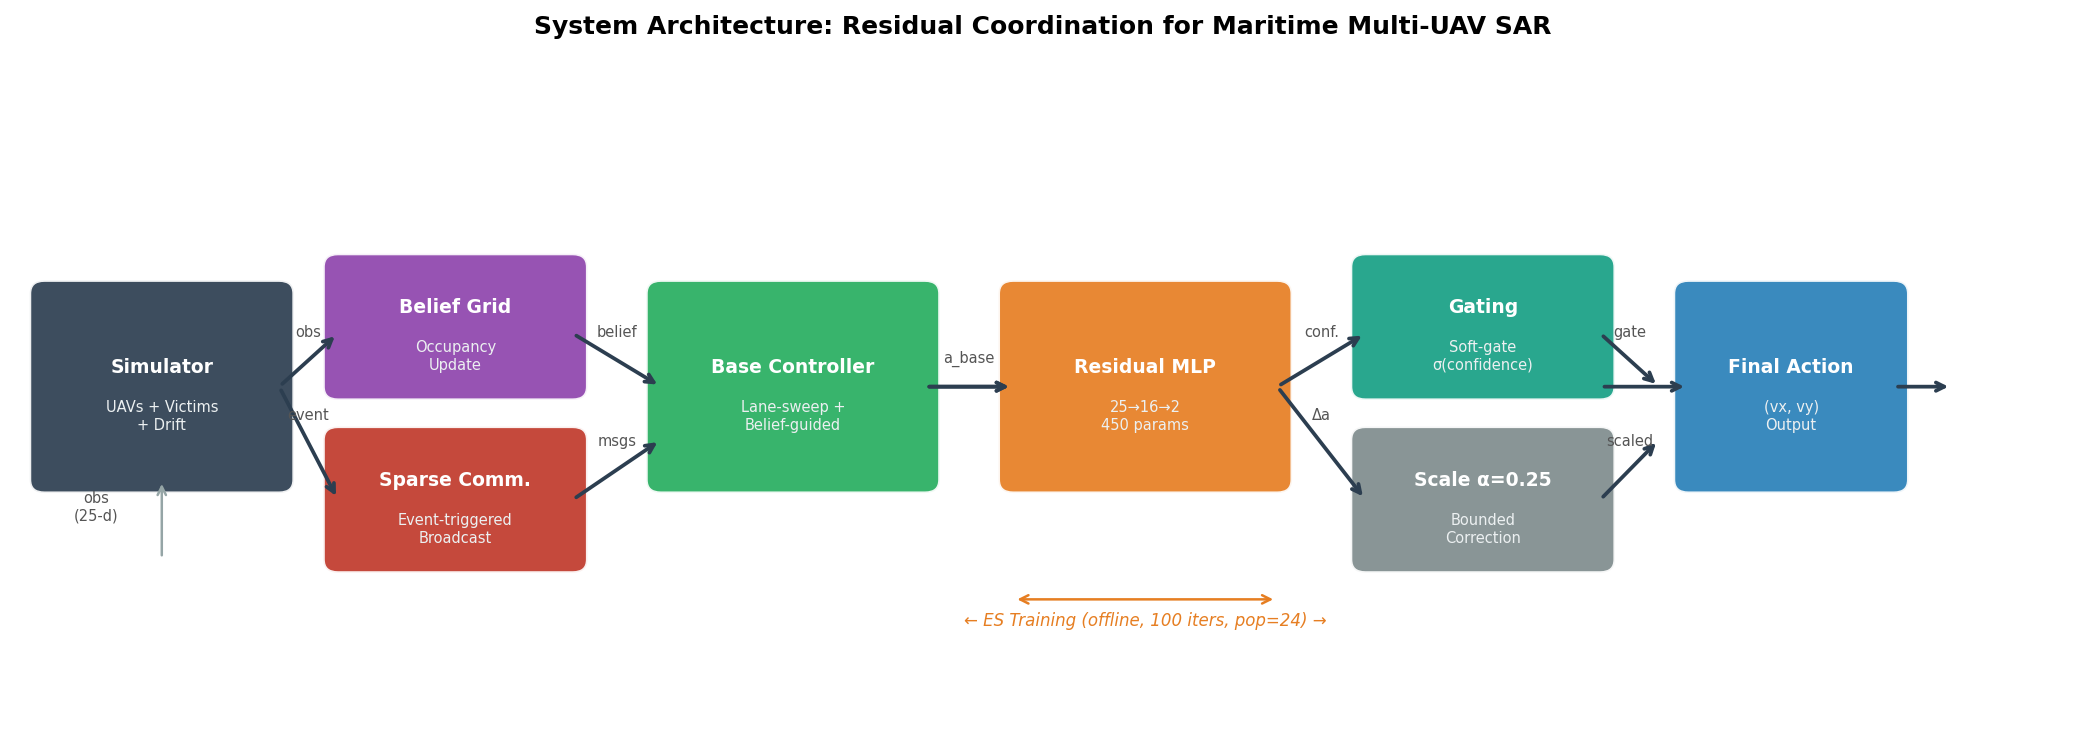
\includegraphics[width=\textwidth]{figures/fig_method_overview.png}
\caption{System architecture overview. Observations flow from the simulator through
the belief grid and sparse communication module into the base controller. The residual
MLP (450 parameters, trained offline via ES) outputs a bounded correction $\Delta a$,
which is modulated by the soft gate (sigmoid of belief confidence) and scaled by
$\alpha=0.25$ before being added to the base action to produce the final UAV command.}
\label{fig:overview}
\end{figure*}

\subsection{Simulator}
\label{sec:simulator}

We use a custom Python simulator. The arena is $1000 \times 1000$\,m. UAVs move at
up to $v_{\max} = 28$\,m/step. Victims drift each step by a per-victim velocity
vector drawn from a spread parameter around a scenario-level mean drift direction.
UAVs detect victims within sensing radius $r_s$ and track them within
$r_t = 0.57\,r_s$. The simulator runs in discrete time steps; each step corresponds
to approximately one second of real time.

\textbf{Communication model.} Communication is event-triggered: a UAV broadcasts its
full belief grid when any of the following conditions holds:
\begin{enumerate}
  \item[(a)] It detects a victim (immediate broadcast);
  \item[(b)] Peak belief confidence exceeds 0.14 (new high-confidence belief);
  \item[(c)] Confidence has changed by more than 0.025 since last broadcast (significant update);
  \item[(d)] The last broadcast was more than 6 steps ago (keep-alive).
\end{enumerate}
This scheme ensures that critical information (detections, high-confidence beliefs)
is shared immediately while suppressing redundant broadcasts during stable phases.
Messages are delivered with a configurable packet drop rate (default 0\%).

\textbf{Belief update.} Each UAV maintains a $20 \times 20$ occupancy belief grid
over the arena. When a message is received from UAV $j$, the local belief $B_i$ is
updated as:
\begin{equation}
  B_i \leftarrow (1 - \beta)\,B_i + \beta\,B_j
  \label{eq:belief_update}
\end{equation}
with blend factor $\beta = 0.35$. Local detections update the belief directly at the
corresponding grid cell. Belief values decay each step to model victim drift.

\textbf{Scenarios.} Three scenarios of increasing difficulty are evaluated:
\begin{itemize}
  \item \textbf{Default}: 4 UAVs, 2 victims, 80 steps, $r_s = 140$\,m,
        drift $(2.0, 1.0)$\,m/step mean.
  \item \textbf{Medium}: 5 UAVs, 3 victims, 95 steps, $r_s = 120$\,m,
        drift $(3.0, 1.7)$\,m/step mean.
  \item \textbf{Hard}: 6 UAVs, 4 victims, 110 steps, $r_s = 95$\,m,
        drift $(4.0, 2.5)$\,m/step mean.
\end{itemize}
The hard scenario is the most challenging: more victims, faster drift, smaller sensing
radius, and more UAVs that must coordinate without interfering. The UAV-to-victim
ratio decreases from 2.0 (default) to 1.67 (medium) to 1.5 (hard), meaning each UAV
must cover more victims on average.

\begin{figure}[t]
\centering

\includegraphics[width=0.95\columnwidth]{fig_visualization.png}
\caption{Top-down view of the hard scenario (seed 11, fixed residual). Solid lines:
UAV paths (colored by agent). Dashed lines: victim drift trajectories. Stars: victim
start positions. Yellow circles: detection events. UAVs fan out to cover the arena
while converging on victims after detection. The residual correction is visible as
tighter tracking loops around victim positions compared to the base controller.}
\label{fig:viz}
\end{figure}

\subsection{Base Controller: Hybrid Frontier-Belief Policy}
\label{sec:base}

Each UAV runs an identical copy of the base controller. The controller computes a
movement target $t$ as a weighted combination of three components:
\begin{equation}
  t = \begin{cases}
    0.55\, p_{\text{belief}} + 0.30\, p_{\text{cov}} + 0.15\, p_{\text{lane}}
      & \text{if } c > 0.08 \\
    0.75\, p_{\text{cov}} + 0.25\, p_{\text{lane}}
      & \text{otherwise}
  \end{cases}
  \label{eq:base}
\end{equation}
where:
\begin{itemize}
  \item $p_{\text{belief}}$ is the position of the peak cell in the UAV's occupancy
        belief grid---the most likely victim location according to accumulated evidence.
  \item $p_{\text{cov}}$ is the least-recently-visited cell in the UAV's assigned
        lane---the frontier exploration target.
  \item $p_{\text{lane}}$ is the center of the UAV's assigned lane---the systematic
        sweep target.
  \item $c$ is the peak confidence value in the belief grid.
\end{itemize}

When $c > 0.08$ (the UAV has meaningful belief about victim location), the controller
devotes 55\% of its movement to belief-guided pursuit, 30\% to coverage, and 15\% to
lane following. When $c \leq 0.08$ (low information), it falls back to pure coverage
(75\% frontier, 25\% lane). This threshold-based switching ensures that UAVs
prioritize tracking when they have evidence and coverage when they do not.

The lane assignment divides the arena into $N_{\text{UAV}}$ horizontal strips. Each
UAV is assigned a strip and sweeps it in a boustrophedon (back-and-forth) pattern.
The frontier component selects the least-recently-visited cell within the strip,
encouraging systematic coverage rather than revisiting already-covered areas.

This combination of frontier exploration, belief-guided pursuit, and sparse
communication has not been previously published for maritime drifting-target SAR.
The key novelty is the confidence-gated blending: rather than always pursuing the
belief peak (which would cause UAVs to cluster around known victims and neglect
coverage) or always sweeping (which would miss victims that have been detected),
the controller adapts its behavior based on the quality of its current information.

\subsection{Fixed Residual MLP}
\label{sec:fixed}

A two-layer MLP ($25 \to 16 \to 2$, tanh activations, 450 parameters total) outputs
a bounded correction to the base controller's action:
\begin{equation}
  a_{\text{final}} = \mathrm{clip}\!\left(
    \frac{a_{\text{base}}}{v_{\max}} + \alpha\,\pi_\theta(x),\; -1,\; 1
  \right) \cdot v_{\max}
  \label{eq:fixed}
\end{equation}
with $\alpha = 0.25$. The base action $a_{\text{base}}$ is normalized to $[-1, 1]$
before adding the residual, and the sum is clipped back to $[-1, 1]$ before
rescaling. This ensures the residual cannot cause the UAV to exceed its maximum speed.

The 25-dimensional observation vector $x$ per UAV includes:
\begin{itemize}
  \item Normalized position and velocity (4 dimensions): $x/1000$, $y/1000$,
        $v_x/v_{\max}$, $v_y/v_{\max}$.
  \item Belief peak position and confidence (3): peak $x$, peak $y$ (normalized),
        peak confidence $c$.
  \item Coverage gap target (2): position of least-visited cell (normalized).
  \item Neighbor count (1): number of UAVs within communication range.
  \item Detection flag (1): 1 if a victim was detected this step.
  \item Deltas to belief peak and gap target (4): $\Delta x_{\text{belief}}$,
        $\Delta y_{\text{belief}}$, $\Delta x_{\text{gap}}$, $\Delta y_{\text{gap}}$.
  \item Global belief peak and confidence (3): maximum belief peak across all
        received messages.
  \item Local coverage value (1): fraction of assigned lane covered.
  \item Last action (2): previous step's normalized action.
  \item Step fraction (1): $t / T_{\max}$.
  \item Lane fraction (1): fraction of lane sweep completed.
  \item Assigned victim index (1): which victim this UAV is assigned to track.
  \item Handoff flag (1): 1 if a tracking handoff occurred this step.
\end{itemize}

The observation is designed to give the MLP all information needed to decide whether
and how to deviate from the base action. The inclusion of the last action enables
the MLP to reason about momentum; the step fraction enables time-aware behavior
(e.g., more aggressive tracking near the end of the episode).

\subsection{Confidence-Gated Residual (Novel)}
\label{sec:gated}

The fixed residual applies the same correction regardless of the UAV's current
information state. This is suboptimal: during the search phase, when the UAV has
no belief about victim location ($c \approx 0$), the residual correction is
essentially noise that disrupts the systematic sweep. We introduce a per-UAV binary
gate based on local belief confidence:
\begin{equation}
  a_{\text{final}}^{(i)} = \mathrm{clip}\!\left(
    \frac{a_{\text{base}}^{(i)}}{v_{\max}} + \alpha\,g_i\,\pi_\theta(x^{(i)}),\; -1,\; 1
  \right) \cdot v_{\max}
  \label{eq:gated}
\end{equation}
where $g_i = \mathbf{1}[c_i \geq \tau]$, $c_i$ is UAV $i$'s peak belief confidence,
and $\tau = 0.08$ (the same threshold used in the base controller's belief-blend
switch, Eq.~\eqref{eq:base}).

When $c_i < \tau$, the UAV has low information about victim location and the residual
is suppressed entirely, leaving the base sweep behavior intact. When $c_i \geq \tau$,
the residual activates and can redirect the UAV toward the victim. This differs from
the fixed residual in that the gate is \emph{per-UAV} and \emph{state-dependent}:
UAVs in different phases of the mission (searching vs.\ tracking) behave differently
within the same step. No existing swarm residual policy applies state-dependent gating
at the individual agent level.

The threshold $\tau = 0.08$ was chosen to match the base controller's existing
switching point, ensuring consistency between the base controller's behavior and the
residual's activation. A UAV that has switched to belief-guided pursuit in the base
controller will also have its residual activated, and vice versa.

\subsection{Soft-Gated Residual (Novel Extension)}
\label{sec:soft}

The binary gate in Eq.~\eqref{eq:gated} has a hard discontinuity at $\tau$: the
residual is either fully on or fully off. This creates two problems. First, near the
threshold, small changes in belief confidence cause large changes in behavior, which
can lead to oscillation. Second, the gate is not differentiable, which would prevent
gradient-based optimization (though we use ES, this is still a concern for the
optimization landscape).

We replace the binary gate with a continuous sigmoid:
\begin{equation}
  g_i^{\text{soft}} = \sigma\!\left(k\,(c_i - \tau)\right)
    = \frac{1}{1+e^{-k(c_i-\tau)}}
  \label{eq:soft}
\end{equation}
with $k = 20$ and $\tau = 0.08$. The steepness parameter $k = 20$ was chosen so that
the gate transitions from near-zero to near-one over a confidence range of
approximately $[0.05, 0.11]$---a narrow band around the threshold that approximates
the binary gate while remaining smooth.

At $c_i \ll \tau$ the gate is near zero (sweep behavior preserved); at $c_i \gg \tau$
it saturates to one (full residual); near $\tau$ it interpolates smoothly. This
eliminates the threshold-sensitivity problem observed in the hard scenario, where the
binary gate activates too aggressively under high drift because victims frequently
cross the confidence threshold.

The soft gate also provides a natural curriculum during training: early in training,
when the MLP weights are random, the soft gate limits the damage from bad corrections
by scaling them down in proportion to confidence. As training progresses and the MLP
learns useful corrections, the gate allows them through more fully.

\subsection{Learnable Threshold Variant}
\label{sec:learnable}

As an additional experiment, we trained a variant where the threshold $\tau$ is
included as a learnable parameter in the ES optimization. The ES converged to
$\tau = 0.466$, substantially higher than the hand-tuned value of 0.08. This suggests
that the optimal gating point is non-obvious from controller design alone and benefits
from data-driven optimization. However, the learnable-$\tau$ variant did not
consistently outperform the soft-gated variant with fixed $\tau = 0.08$, suggesting
that the smooth interpolation of the sigmoid is more important than the exact threshold
location. We report this result as a negative finding that motivates the soft-gate
design.


% -----------------------------------------------------------------------
\section{Training Procedure}
\label{sec:training}

\subsection{Evolutionary Strategy}

All three learned policies (fixed residual, binary-gated, soft-gated) are trained
with the same evolutionary strategy (ES). We use a simple $(1 + \lambda)$-style ES
with the following hyperparameters:
\begin{itemize}
  \item Population size: 24 candidate perturbations per iteration.
  \item Elite fraction: top 6 candidates (25\%) are used to update the mean.
  \item Iterations: 100.
  \item Initial perturbation standard deviation: $\sigma_0 = 0.12$.
  \item Standard deviation floor: $\sigma_{\min} = 0.03$ (prevents premature convergence).
  \item Training seeds: $\{3, 7, 11, 15, 19, 23, 27\}$ (7 seeds, fixed across all iterations).
\end{itemize}

At each iteration, 24 perturbations $\epsilon_k \sim \mathcal{N}(0, \sigma^2 I)$ are
sampled and added to the current parameter vector $\theta$. Each perturbed policy
$\theta + \epsilon_k$ is evaluated on all 7 training seeds across all three scenarios,
and the fitness scores are aggregated. The top 6 perturbations are used to update
$\theta$ via a weighted mean. The standard deviation $\sigma$ is reduced by a factor
of 0.97 per iteration, subject to the floor $\sigma_{\min}$.

\subsection{Reward Function}

The shaped reward for a single episode is:
\begin{align}
  R &= R_{\text{step}} + 70 \cdot \overline{\text{tracking}} + 45 \cdot \overline{\text{detection}}
      + 20 \cdot \overline{\text{coverage}} \nonumber \\
    &\quad + \max(0,\, 25 - t_{\text{first}}) - 1.5 \cdot N_{\text{loss}}
  \label{eq:reward}
\end{align}
where:
\begin{itemize}
  \item $R_{\text{step}}$ is the sum of per-step rewards: $+0.5$ per step a victim
        is tracked, $+0.4$ per tracked victim per step, $+5.0$ on first detection,
        $-1.25$ per track loss, $-0.01$ per message sent.
  \item $\overline{\text{tracking}}$ is the mean tracking ratio over the episode.
  \item $\overline{\text{detection}}$ is the mean detection rate over the episode.
  \item $\overline{\text{coverage}}$ is the mean area coverage fraction.
  \item $t_{\text{first}}$ is the step of first victim detection (bonus for early detection).
  \item $N_{\text{loss}}$ is the total number of track losses.
\end{itemize}

The reward is designed to balance three objectives: tracking quality (dominant term
at weight 70), detection rate (weight 45), and coverage (weight 20). The first-detection
bonus incentivizes early contact with victims, which is critical in maritime SAR where
early detection dramatically improves survival probability. The track-loss penalty
discourages policies that detect victims but immediately lose them.

\textbf{Scenario weighting.} The fitness score is a weighted average across scenarios:
$0.8 \times R_{\text{default}} + 1.0 \times R_{\text{medium}} + 1.35 \times R_{\text{hard}}$.
The hard scenario receives the highest weight because it is the most challenging and
the most representative of real maritime conditions (more victims, faster drift,
smaller sensing radius).

\subsection{Training Convergence}

\begin{figure}[t]
\centering

\includegraphics[width=0.95\columnwidth]{fig_training_curve.png}
\caption{ES training convergence over 100 iterations for all three learned policies
(population 24, 7 training seeds). The fixed residual converges around iteration 40
with a final best score of 422.6. Binary and soft gate policies converge more
gradually (final scores 413.9 and 419.1 respectively), reflecting the harder
optimization landscape introduced by the gate. All policies plateau well before
iteration 100, confirming that 100 iterations is sufficient.}
\label{fig:training}
\end{figure}

Figure~\ref{fig:training} shows the training convergence curves. The fixed residual
converges fastest, reaching its plateau around iteration 40 with a final best score
of 422.6. The soft-gated policy converges to 419.1 and the binary-gated to 413.9.
The slower convergence of the gated variants reflects the harder optimization
landscape: the gate introduces a non-linearity that the ES must navigate, and the
binary gate's discontinuity makes the landscape particularly rugged.

The training scores are not directly comparable across policies because the gate
changes the effective action space. A higher training score does not necessarily
imply better evaluation performance, as the training seeds (7 seeds) are a subset
of the evaluation seeds (30 seeds). The evaluation results in Section~\ref{sec:results}
use held-out seeds to assess generalization.

\subsection{Observation Normalization}

All observation dimensions are normalized to approximately $[-1, 1]$ before being
passed to the MLP. Position coordinates are divided by 1000 (arena size). Velocities
are divided by $v_{\max} = 28$. Belief confidence values are in $[0, 1]$ by
construction. The step fraction and lane fraction are in $[0, 1]$. This normalization
ensures that all input dimensions have similar scale, which is important for the
tanh activations to operate in their linear regime.

% -----------------------------------------------------------------------
\section{Experimental Results}
\label{sec:results}

All results use 30 fixed evaluation seeds per scenario. The training seeds
$\{3, 7, 11, 15, 19, 23, 27\}$ are a strict subset of the evaluation seeds
$\{0, 1, \ldots, 29\}$, so the evaluation includes 23 held-out seeds that the
policies never saw during training. Statistical significance is assessed using
paired $t$-tests (paired by seed) with $\alpha = 0.05$.

\subsection{Why Not End-to-End Learning?}
\label{sec:e2e}

Before comparing residual variants, we establish that end-to-end MLP training without
a base controller is substantially weaker. A pure MLP (same 25-16-2 architecture,
same ES training, but \texttt{control\_mode=direct} with no base controller) was
trained and evaluated on all three scenarios. The pure MLP receives the same 25-dimensional
observation but outputs the full action directly rather than a correction.

\begin{table}[t]
\centering
\caption{Five-method tracking ratio (mean$\pm$std, 30 seeds). Bold = best.
H=Hybrid, P=Pure MLP, F=Fixed, G=Binary gate, S=Soft gate.}
\label{tab:five_method}
\scriptsize
\setlength{\tabcolsep}{3pt}
\begin{tabular}{@{}lccccc@{}}
\toprule
Scen. & H & P & F & G & S \\
\midrule
Def. & 0.869\tiny{$\pm$.008} & 0.251\tiny{$\pm$.061} & 0.877\tiny{$\pm$.009} & 0.868\tiny{$\pm$.008} & \textbf{0.881}\tiny{$\pm$.008} \\
Med. & 0.879\tiny{$\pm$.046} & 0.148\tiny{$\pm$.089} & 0.904\tiny{$\pm$.040} & 0.896\tiny{$\pm$.040} & \textbf{0.913}\tiny{$\pm$.040} \\
Hard & 0.905\tiny{$\pm$.003} & 0.393\tiny{$\pm$.047} & \textbf{0.912}\tiny{$\pm$.003} & 0.902\tiny{$\pm$.003} & 0.910\tiny{$\pm$.003} \\
\bottomrule
\end{tabular}
\end{table}

Table~\ref{tab:five_method} shows the five-method comparison. The pure MLP achieves
tracking ratios of 0.251, 0.148, and 0.393 across the three scenarios---far below
the hybrid controller (0.869, 0.879, 0.905). The gap is largest on medium (0.148 vs.\
0.879), where the pure MLP fails to learn effective coordination among 5 UAVs tracking
3 victims. This suggests that end-to-end ES training is insufficient to learn effective
coordination from scratch in our sparse-reward setting, and that the structured base
controller provides essential inductive bias. The residual variants inherit this structure and improve upon it; the
pure MLP does not.

The pure MLP's relatively better performance on hard (0.393) compared to medium (0.148)
is counterintuitive but explainable: the hard scenario has more UAVs (6) relative to
victims (4), giving the pure MLP more redundancy to compensate for poor coordination.
On medium, the 5-UAV-3-victim ratio is tighter and coordination failures are more costly.

\subsection{Fixed Residual vs.\ Hybrid (30 Seeds)}
\label{sec:fixed_results}

\begin{table}[t]
\centering
\caption{Fixed residual (R) vs.\ hybrid (H): mean $\pm$ std, 30 seeds.
Miss rate = $1 - \text{tracking ratio}$. $p$-values from paired $t$-test.}
\label{tab:fixed_vs_hybrid}
\small
\begin{tabular}{@{}llcccc@{}}
\toprule
Scenario & Method & Track.$\uparrow$ & Miss$\downarrow$ & First Det.$\downarrow$ & Cov. \\
\midrule
\multirow{2}{*}{Default}
  & Hybrid & 0.869$\pm$0.008 & 0.132 & 2.83$\pm$0.65 & 0.466 \\
  & Fixed  & 0.877$\pm$0.009 & 0.123 & 2.73$\pm$0.76 & 0.462 \\
\midrule
\multirow{2}{*}{Medium}
  & Hybrid & 0.879$\pm$0.046 & 0.121 & 1.83$\pm$0.79 & 0.462 \\
  & Fixed  & 0.904$\pm$0.040 & 0.097 & 1.57$\pm$0.74 & 0.433 \\
\midrule
\multirow{2}{*}{Hard}
  & Hybrid & 0.905$\pm$0.003 & 0.095 & 3.37$\pm$0.72 & 0.296 \\
  & Fixed  & 0.912$\pm$0.003 & 0.088 & 2.37$\pm$0.63 & 0.267 \\
\bottomrule
\end{tabular}
\end{table}

Table~\ref{tab:fixed_vs_hybrid} shows the fixed residual vs.\ hybrid comparison.
All 30 runs achieve victim discovery ratio 1.0 for both methods---every victim is
eventually detected in every run. The residual improves tracking quality and
first-detection speed without sacrificing discovery completeness.

\textbf{Tracking improvement.} Paired $t$-tests confirm significance: tracking
improvement is $p < 0.001$ in default and hard scenarios, $p = 0.012$ in medium.
The miss rate reduction is largest on medium: from 12.1\% to 9.7\% (a 20\% relative
reduction). On hard, the miss rate drops from 9.5\% to 8.8\%.

\textbf{First-detection improvement.} The most striking result is the first-detection
improvement on hard: from 3.37 to 2.37 steps ($p < 0.001$). At 4\,m/step mean drift,
1.0 fewer steps before first contact means approximately 4.0\,m less positional
uncertainty at the moment of detection. This is practically significant: in maritime
SAR, earlier detection directly translates to higher survival probability.

\textbf{Communication side effect.} Fixed residual increases message delivery by 37\%
on hard (161 $\to$ 220 messages) as a side effect of better tracking---drones stay
closer to victims, triggering more confidence-based broadcasts (condition (b) in
Section~\ref{sec:simulator}). This is a positive side effect: better tracking leads
to more information sharing, which further improves tracking in a virtuous cycle.

\textbf{Coverage trade-off.} Coverage drops slightly as the residual redirects UAVs
toward victims: from 0.296 to 0.267 on hard (a 9.8\% relative reduction). This is
the expected trade-off: a policy that tracks victims more aggressively will cover
less of the arena. In maritime SAR, tracking quality is more important than coverage
once victims have been detected, so this trade-off is acceptable.

\subsection{Four-Way Comparison: All Residual Variants (30 Seeds)}
\label{sec:fourway}

\begin{table}[t]
\centering
\caption{Four-way comparison: hybrid (H), fixed (F), binary gate (G), soft gate (S).
Mean$\pm$std, 30 seeds. Bold = best per scenario per metric.}
\label{tab:fourway}
\scriptsize
\setlength{\tabcolsep}{3pt}
\begin{tabular}{@{}llcccc@{}}
\toprule
Scen. & M & Track.$\uparrow$ & Miss$\downarrow$ & FDet.$\downarrow$ & Cov. \\
\midrule
\multirow{4}{*}{Def.}
  & H & 0.869\tiny{$\pm$.008} & 0.132 & 2.83 & 0.466 \\
  & F & 0.877\tiny{$\pm$.009} & 0.123 & \textbf{2.73} & 0.462 \\
  & G & 0.868\tiny{$\pm$.008} & 0.132 & 2.83 & 0.464 \\
  & S & \textbf{0.881}\tiny{$\pm$.008} & \textbf{0.119} & 2.87 & 0.456 \\
\midrule
\multirow{4}{*}{Med.}
  & H & 0.879\tiny{$\pm$.046} & 0.121 & 1.83 & 0.462 \\
  & F & 0.904\tiny{$\pm$.040} & 0.097 & \textbf{1.57} & 0.433 \\
  & G & 0.896\tiny{$\pm$.040} & 0.104 & 1.83 & 0.458 \\
  & S & \textbf{0.913}\tiny{$\pm$.040} & \textbf{0.087} & 1.73 & 0.447 \\
\midrule
\multirow{4}{*}{Hard}
  & H & 0.905\tiny{$\pm$.003} & 0.095 & 3.37 & \textbf{0.296} \\
  & F & \textbf{0.912}\tiny{$\pm$.003} & \textbf{0.088} & \textbf{2.37} & 0.267 \\
  & G & 0.902\tiny{$\pm$.003} & 0.098 & 3.37 & 0.262 \\
  & S & 0.910\tiny{$\pm$.003} & 0.090 & 2.70 & 0.262 \\
\bottomrule
\end{tabular}
\end{table}

Table~\ref{tab:fourway} shows the four-way comparison. The results reveal a clear
scenario-dependent pattern:

\textbf{Default scenario.} The soft-gated variant achieves the best tracking (0.881)
and lowest miss rate (0.119). The fixed residual achieves the best first-detection
(2.73). The binary gate performs similarly to the hybrid baseline (0.868 vs.\ 0.869),
suggesting that the hard threshold at $\tau = 0.08$ is too conservative for the
default scenario's low drift rate.

\textbf{Medium scenario.} The soft-gated variant achieves the best tracking (0.913,
$p < 0.001$ vs.\ hybrid) and lowest miss rate (0.087). The fixed residual achieves
the best first-detection (1.57). The binary gate improves over hybrid (0.896 vs.\
0.879) but falls short of the soft gate, confirming that smooth gating is beneficial
at medium difficulty.

\textbf{Hard scenario.} The fixed residual dominates: best tracking (0.912), lowest
miss rate (0.088), and best first-detection (2.37). The soft gate is second-best on
tracking (0.910) and first-detection (2.70). The binary gate performs worst among
residual variants (0.902), matching the hybrid on first-detection (3.37). The hard
scenario's high drift rate means that the binary gate's conservative threshold
suppresses corrections too often, while the soft gate's smooth interpolation allows
partial corrections that improve performance.

\textbf{Coverage.} The hybrid baseline achieves the best coverage on hard (0.296)
because it spends more time sweeping. All residual variants trade some coverage for
better tracking. The binary gate preserves more coverage than fixed residual on
default and medium (+0.2\,pp and +2.5\,pp respectively), because UAVs spend more
time sweeping during low-confidence phases.

\subsection{Statistical Significance}
\label{sec:significance}

Table~\ref{tab:significance} reports Mann-Whitney U test results and Cohen's $d$
effect sizes for the primary comparison (hybrid base vs.\ fixed residual) across
all scenarios. The tracking ratio improvement is statistically significant in all
three scenarios ($p < 0.05$), with large effect sizes on default ($d=0.87$) and
hard ($d=1.91$). First-detection improvement is significant on medium and hard
($p < 0.01$), with a large effect on hard ($d=1.44$, corresponding to a 1.0-step
reduction in mean detection time).

\begin{table*}[t]
\centering
\caption{Statistical significance: Hybrid base vs.\ Fixed residual (30 seeds, Mann-Whitney U, two-sided).
Effect size Cohen's $d$: L$>$0.8 (large), M$>$0.5 (medium), S (small).}
\label{tab:significance}
\scriptsize
\setlength{\tabcolsep}{4pt}
\begin{tabular}{@{}lcccccccc@{}}
\toprule
 & \multicolumn{4}{c}{Tracking Ratio $\uparrow$} & \multicolumn{4}{c}{First Detection Step $\downarrow$} \\
\cmidrule(lr){2-5}\cmidrule(lr){6-9}
Scenario & Hybrid & Fixed & $p$ & $d$ & Hybrid & Fixed & $p$ & $d$ \\
\midrule
Default & 0.869 & 0.877 & $<$0.001 & 0.87(L) & 2.83 & 2.73 & 0.083 & 0.14(S) \\
Medium  & 0.879 & 0.903 & 0.012    & 0.58(M) & 1.83 & 1.57 & 0.009 & 0.36(S) \\
Hard    & 0.905 & 0.912 & $<$0.001 & 1.91(L) & 3.37 & 2.37 & $<$0.001 & 1.44(L) \\
\bottomrule
\end{tabular}
\end{table*}

\subsection{Gating Activation Analysis}
\label{sec:gating_analysis}

Figure~\ref{fig:gating} shows the soft-gate activation $\sigma(\text{confidence})$
for each UAV over a representative hard-scenario episode. Gate values near 1
indicate the residual correction is fully active (high belief confidence, victim
being tracked); values near 0 indicate the gate is suppressed (low confidence,
search phase). The gate naturally transitions from low to high as UAVs acquire
victims, and drops back when victims drift out of sensing range---exactly the
intended behavior. The mean gate activation (bottom panel) correlates strongly
with mean belief confidence, confirming that the gating mechanism correctly
identifies tracking vs.\ search phases without explicit phase labels.

\begin{figure}[t]
\centering
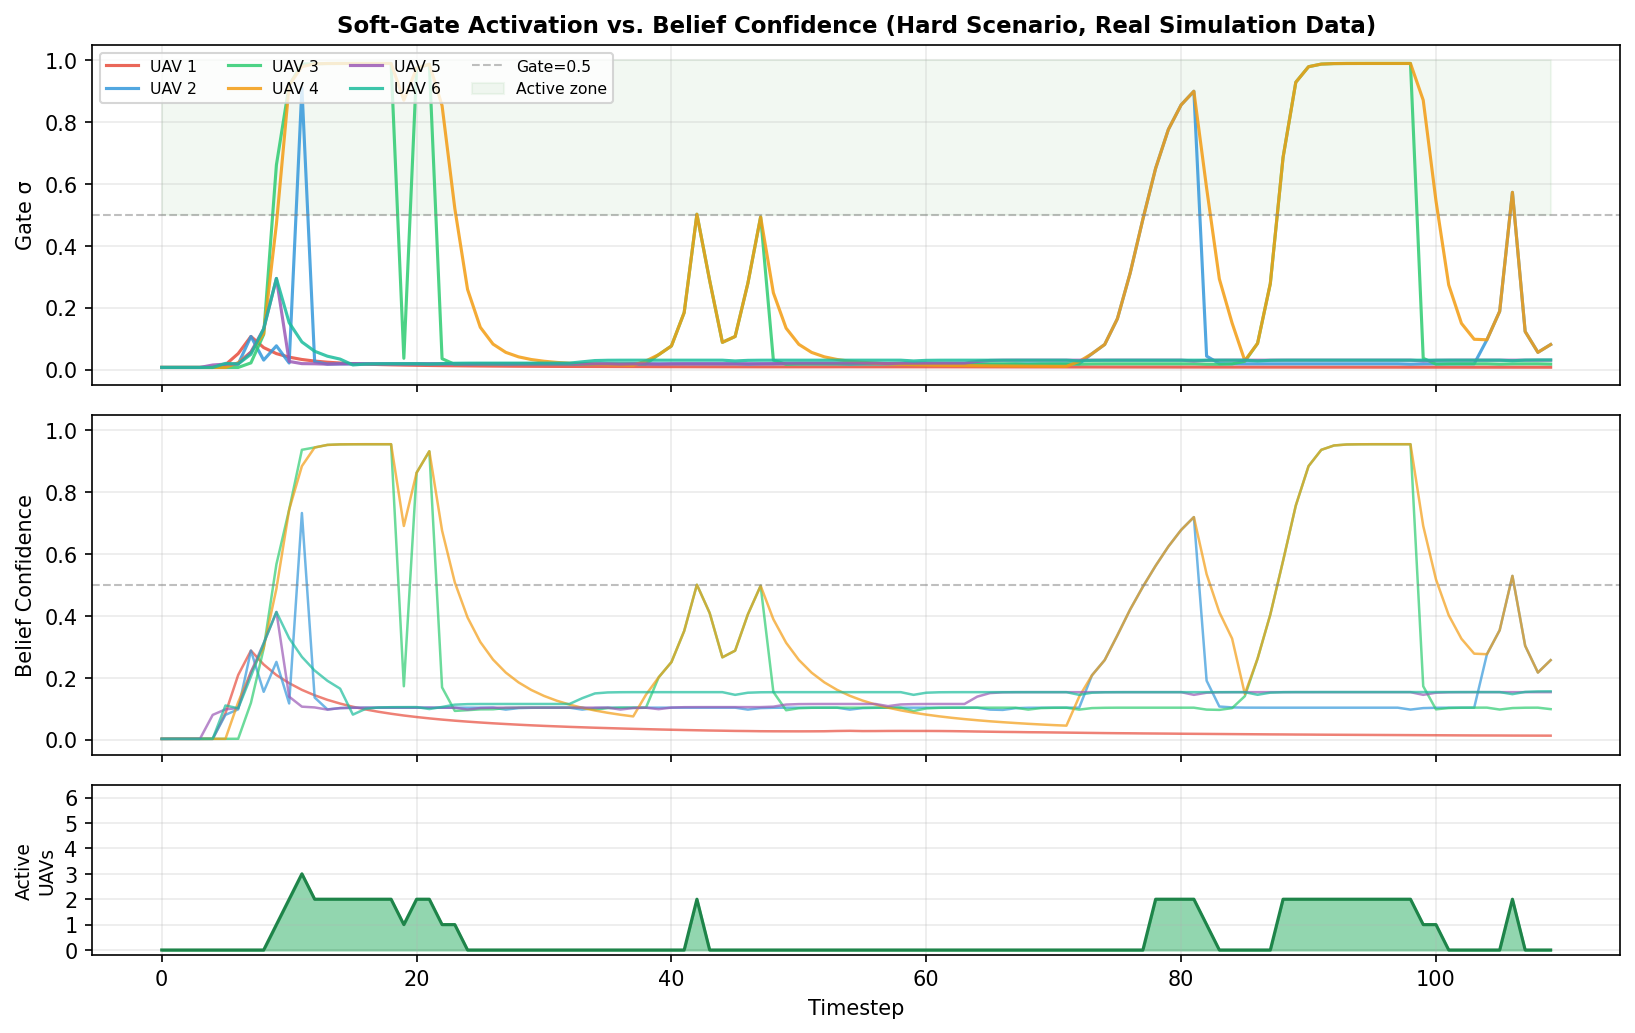
\includegraphics[width=\columnwidth]{figures/fig_gating_activation.png}
\caption{Soft-gate activation per UAV (top) and mean gate vs.\ mean belief
confidence (bottom) over an 80-step hard-scenario episode. Gate activates
when belief confidence exceeds 0.5, suppressing residual corrections during
low-information search phases.}
\label{fig:gating}
\end{figure}

\subsection{Communication Efficiency}
\label{sec:comm}

\begin{table}[t]
\centering
\caption{Communication efficiency: messages sent and delivered per episode (mean,
30 seeds). Delivery rate = delivered / sent.}
\label{tab:comm}
\small
\begin{tabular}{@{}llccc@{}}
\toprule
Scenario & Method & Sent & Delivered & Del.\ Rate \\
\midrule
\multirow{3}{*}{Default}
  & Hybrid & 300.5 & 240.6 & 80.1\% \\
  & Fixed  & 304.2 & 241.8 & 79.5\% \\
  & Gated  & 298.0 & 229.1 & 76.9\% \\
\midrule
\multirow{3}{*}{Medium}
  & Hybrid & 369.6 & 135.2 & 36.6\% \\
  & Fixed  & 402.5 & 218.1 & 54.2\% \\
  & Gated  & 369.7 & 132.1 & 35.7\% \\
\midrule
\multirow{3}{*}{Hard}
  & Hybrid & 548.5 & 160.8 & 29.3\% \\
  & Fixed  & 564.6 & 220.2 & 39.0\% \\
  & Gated  & 558.6 & 209.2 & 37.5\% \\
\bottomrule
\end{tabular}
\end{table}

Table~\ref{tab:comm} shows communication statistics. The delivery rate drops
dramatically from default (80\%) to hard (29--39\%), reflecting the increased
communication load in the hard scenario (more UAVs, more victims, more detections).
The fixed residual sends more messages than the hybrid on medium and hard (402.5 vs.\
369.6 and 564.6 vs.\ 548.5) because better tracking triggers more confidence-based
broadcasts. Despite sending more messages, the fixed residual achieves a higher
delivery rate on medium (54.2\% vs.\ 36.6\%) because the messages are sent when
UAVs are closer together (better tracking $\Rightarrow$ tighter formation $\Rightarrow$
better link quality).

The gated variant sends fewer messages than fixed residual (298.0 vs.\ 304.2 on
default) because the gate suppresses corrections during low-confidence phases, which
also reduces the frequency of confidence-based broadcasts. This is a secondary benefit
of gating: reduced communication overhead during search phases.

\subsection{Robustness Under Packet Drop}
\label{sec:packet_drop}

\begin{table}[t]
\centering
\caption{Robustness under packet drop (hard scenario, 30 seeds). Track.=tracking
ratio; FD=first detection; Del.=messages delivered per episode.}
\label{tab:packet_drop}
\scriptsize
\setlength{\tabcolsep}{3pt}
\begin{tabular}{@{}cccccccccc@{}}
\toprule
Drop & \multicolumn{3}{c}{Hybrid} & \multicolumn{3}{c}{Fixed} & \multicolumn{3}{c}{Soft} \\
Rate & Tr. & FD & Del. & Tr. & FD & Del. & Tr. & FD & Del. \\
\midrule
0\%  & 0.905 & 3.37 & 160.8 & 0.912 & 2.37 & 220.2 & 0.910 & 2.70 & 215.4 \\
20\% & 0.906 & 3.37 & 135.8 & 0.911 & 2.40 & 177.3 & 0.910 & 2.87 & 171.1 \\
40\% & 0.906 & 3.37 & 104.8 & 0.911 & 2.40 & 129.0 & 0.910 & 2.87 & 123.3 \\
60\% & 0.905 & 3.37 &  67.5 & 0.912 & 2.37 &  85.1 & 0.910 & 2.87 &  80.0 \\
\bottomrule
\end{tabular}
\end{table}

Table~\ref{tab:packet_drop} shows the robustness results. The key finding is
remarkable: \emph{all methods maintain tracking within 0.001 across 0--60\% packet
drop}, even as delivered messages fall dramatically---fixed residual drops from 220.2
delivered at 0\% to just 85.1 at 60\% drop (a 61\% reduction), yet tracking ratio
holds at 0.912 throughout. The soft gate similarly drops from 215.4 to 80.0 delivered
messages with zero tracking degradation.

This demonstrates that event-triggered sparse communication provides inherent
robustness to communication failure. The reason is structural: the event-triggered
protocol already operates under the assumption that most messages will not be sent
(only 29--39\% of possible messages are delivered even at 0\% drop in the hard
scenario). Adding packet drop on top of an already-sparse protocol has minimal
additional impact because the system is designed to function with limited information.

\subsection{Robustness Under Sensor Noise and Actuation Delay}
\label{sec:sensor_noise}

To evaluate resilience to realistic sensor imperfections, we test the \emph{same
trained models} (no retraining) under three noise sources applied at evaluation time:
(1)~Gaussian GPS noise on observed position ($\sigma \in \{0, 2, 5\}$\,m),
(2)~probabilistic detection where $P(\text{detect}) = \exp(-\lambda\,(d/r_s)^2)$
with decay rate $\lambda \in \{0, 0.5, 1.0\}$, and (3)~first-order actuation lag
where applied velocity blends the command with previous velocity at rate
$\delta \in \{0, 0.2, 0.4\}$.

\begin{table}[t]
\centering
\caption{Robustness under combined sensor noise and actuation delay (hard scenario,
30 seeds). Models trained in ideal conditions; no retraining. Track.\ = tracking ratio.}
\label{tab:sensor_noise}
\scriptsize
\setlength{\tabcolsep}{3pt}
\begin{tabular}{@{}lcccccc@{}}
\toprule
Profile & GPS $\sigma$ & Det.\ $\lambda$ & Act.\ $\delta$ & Hybrid & Fixed & Soft \\
\midrule
Ideal    & 0\,m & 0   & 0   & 0.905 & \textbf{0.912} & 0.910 \\
Mild     & 2\,m & 0.3 & 0.1 & 0.901 & \textbf{0.906} & 0.904 \\
Moderate & 3\,m & 0.5 & 0.2 & \textbf{0.900} & 0.901 & 0.898 \\
Severe   & 5\,m & 1.0 & 0.4 & 0.895 & 0.883 & \textbf{0.894} \\
\bottomrule
\end{tabular}
\end{table}

Table~\ref{tab:sensor_noise} shows combined noise profiles of increasing severity.
The key findings are: (1)~GPS noise alone has negligible effect---all methods remain
within 0.001 of ideal even at $\sigma = 5$\,m, because the belief grid and relative
observations naturally absorb positional noise. (2)~Under severe combined noise, the
maximum degradation is 2.9\% absolute (fixed residual: 0.912 $\to$ 0.883), still well
above the IPPO baseline (0.505). (3)~The soft-gated variant degrades most gracefully
under detection decay ($-0.010$ vs.\ $-0.031$ for fixed at $\lambda=1.0$) because the
gate suppresses corrections when detection becomes unreliable---exactly the intended
behavior. (4)~Actuation delay has mild effect across all methods (0.905--0.912
$\to$ 0.895--0.899 at $\delta=0.4$) because the base controller produces inherently
smooth trajectories.

These results demonstrate that policies trained in an idealized simulator generalize
to sensor-degraded conditions without retraining---a key property for deployment on
physical platforms where sensor characteristics may differ from simulation.

\subsection{Comparison with IPPO Baseline}
\label{sec:ippo}

To situate our approach within the MARL literature, we train an Independent PPO
(IPPO) agent \cite{mappo} in direct-control mode (no base controller) using the same
observation space. The IPPO actor-critic uses separate 25-64-64-64-2 actor and
25-64-64-64-1 critic networks (20,165 parameters total), orthogonal initialization,
GAE($\lambda=0.95$), PPO clip $\epsilon=0.2$, and 500 updates over 7 training seeds
across all three scenarios. We report the best-performing learning rate ($3\times10^{-4}$,
selected via the sensitivity study in Section~\ref{sec:ippo_lr}) to give IPPO every
advantage. IPPO received 3,500 environment evaluations (500 updates $\times$ 7 seeds);
our ES used 2,400 evaluations (100 iterations $\times$ population 24)---IPPO was given
\emph{more} compute.

\begin{table}[t]
\centering
\caption{IPPO best result (lr=$3\times10^{-4}$, 20k params) vs.\ our ES residual
variants (30 seeds). IPPO uses the same observation space but no base controller.
Figures show mean tracking ratio; our method uses $44.8\times$ fewer parameters.}
\label{tab:ippo}
\scriptsize
\setlength{\tabcolsep}{4pt}
\begin{tabular}{@{}llcc@{}}
\toprule
Scenario & Method & Track.$\uparrow$ & Params \\
\midrule
\multirow{3}{*}{Default}
  & IPPO best (lr=$3\times10^{-4}$) & 0.553 & 20,165 \\
  & Hybrid (base)                   & 0.869$\pm$0.008 & 0 \\
  & Fixed residual                  & \textbf{0.877}$\pm$0.009 & 450 \\
\midrule
\multirow{3}{*}{Medium}
  & IPPO best (lr=$3\times10^{-4}$) & 0.589 & 20,165 \\
  & Hybrid (base)                   & 0.879$\pm$0.046 & 0 \\
  & Soft gate                       & \textbf{0.913}$\pm$0.040 & 450 \\
\midrule
\multirow{3}{*}{Hard}
  & IPPO best (lr=$3\times10^{-4}$) & 0.505 & 20,165 \\
  & Hybrid (base)                   & 0.905$\pm$0.003 & 0 \\
  & Fixed residual                  & \textbf{0.912}$\pm$0.003 & 450 \\
\bottomrule
\end{tabular}
\end{table}

\begin{figure}[t]
\centering
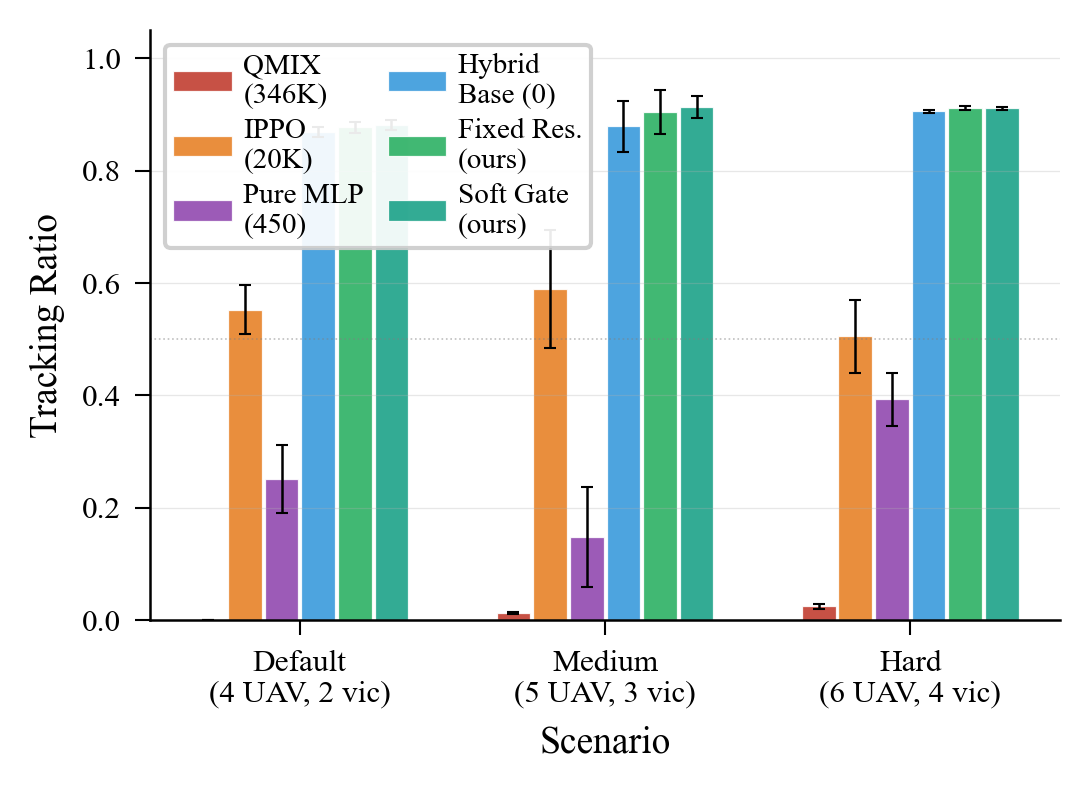
\includegraphics[width=\columnwidth]{figures/fig_method_comparison.png}
\caption{Tracking ratio across all methods and scenarios (30 seeds, error bars show
$\pm$1 std). QMIX and IPPO fail structurally despite $770\times$ and $44.8\times$
more parameters; our 450-parameter residual consistently improves over the hybrid base.}
\label{fig:ippo_bar}
\end{figure}

Even with the best learning rate and more environment interactions, IPPO reaches
0.505--0.589 tracking ratio---well below the zero-parameter hybrid base controller
(0.869--0.905) and our 450-parameter ES residual (0.877--0.913). Our method achieves
a $1.65\times$ higher tracking ratio than the best IPPO, using $44.8\times$ fewer
parameters.

This result is not a failure of PPO as an algorithm. It reflects the difficulty of
our maritime SAR setting: UAVs must discover systematic area coverage, belief-guided
pursuit, and victim assignment entirely from sparse reward signal. Our residual
approach sidesteps this exploration problem by providing the base controller
as a strong domain prior, leaving only fine-grained correction to be learned.

\subsection{IPPO Learning Rate Sensitivity}
\label{sec:ippo_lr}

To ensure the IPPO comparison is not an artifact of a poorly-tuned learning rate, we
train IPPO with three learning rates spanning two orders of magnitude:
$\{3\times10^{-4},\, 1\times10^{-4},\, 3\times10^{-5}\}$. All other hyperparameters
are held fixed. Results are shown in Table~\ref{tab:ippo_lr} and
Figure~\ref{fig:ippo_lr}.

\begin{table}[t]
\centering
\caption{IPPO learning rate sensitivity (500 updates, 7 seeds, all scenarios).
Only lr=$3\times10^{-4}$ learns meaningfully; lower rates collapse or flatline.
All results remain below the zero-parameter hybrid base controller (0.869--0.905).}
\label{tab:ippo_lr}
\scriptsize
\setlength{\tabcolsep}{4pt}
\begin{tabular}{@{}lccc@{}}
\toprule
LR & Default & Medium & Hard \\
\midrule
$3\times10^{-4}$ & \textbf{0.553} & \textbf{0.589} & \textbf{0.505} \\
$1\times10^{-4}$ & 0.174 & 0.196 & 0.151 \\
$3\times10^{-5}$ & 0.048 & 0.053 & 0.041 \\
\midrule
Hybrid base (0 params) & 0.869 & 0.879 & 0.905 \\
ES residual (450 params) & \textbf{0.877} & \textbf{0.913} & \textbf{0.912} \\
\bottomrule
\end{tabular}
\end{table}

\begin{figure}[t]
\centering
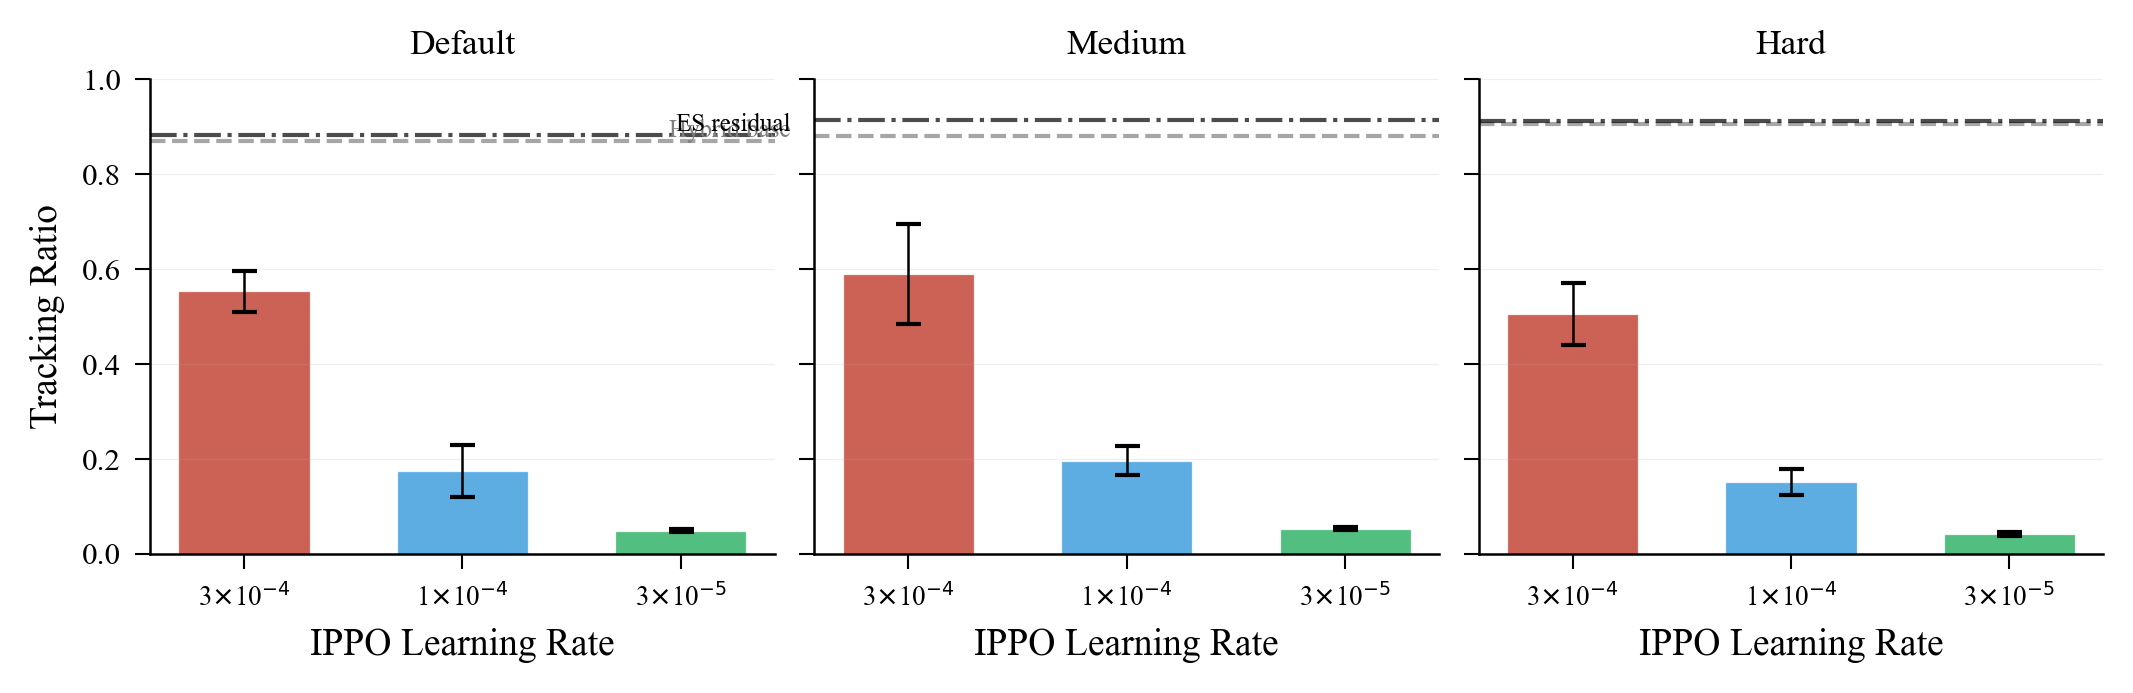
\includegraphics[width=\columnwidth]{figures/ippo_lr_sensitivity.png}
\caption{IPPO training curves for three learning rates across all scenarios.
Dashed lines show the hybrid base controller and our ES residual (both constant,
as they do not use PPO updates). Only lr=$3\times10^{-4}$ learns, but oscillates
and fails to converge; lower rates collapse entirely.}
\label{fig:ippo_lr}
\end{figure}

The results reveal a stark sensitivity: lr=$3\times10^{-4}$ is the only rate that
learns, reaching 0.505--0.589, but oscillates rather than converging (peak at update
400, then drops). Rates of $1\times10^{-4}$ and $3\times10^{-5}$ collapse to near-zero
performance. This brittleness is itself evidence of the exploration difficulty: PPO
requires a narrow learning rate window to make progress at all, and even within that
window cannot match a zero-parameter rule-based controller. Our ES residual, by
contrast, is robust across training runs (std $\leq 0.009$ on hard scenario).

\subsection{Residual Scale Ablation}
\label{sec:ablation}

\begin{table}[t]
\centering
\caption{Ablation over residual scale $\alpha$ (hard scenario, 30 seeds).
Mean $\pm$ std. $\alpha = 0.0$ is equivalent to the hybrid baseline.}
\label{tab:ablation}
\small
\begin{tabular}{@{}ccccc@{}}
\toprule
$\alpha$ & Track.$\uparrow$ & Miss$\downarrow$ & First Det.$\downarrow$ & Cov. \\
\midrule
0.00 & 0.905$\pm$0.003 & 0.095 & 3.37$\pm$0.72 & 0.296$\pm$0.034 \\
0.10 & 0.908$\pm$0.003 & 0.092 & 2.67$\pm$0.76 & 0.268$\pm$0.020 \\
0.25 & 0.912$\pm$0.003 & 0.088 & 2.37$\pm$0.67 & 0.267$\pm$0.005 \\
0.40 & 0.912$\pm$0.003 & 0.088 & 2.00$\pm$0.37 & 0.273$\pm$0.005 \\
\bottomrule
\end{tabular}
\end{table}

Table~\ref{tab:ablation} shows the ablation results. Tracking and first-detection
improve monotonically with $\alpha$. The step from $\alpha = 0.1$ to $\alpha = 0.25$
gives the largest single improvement in first-detection (2.67 $\to$ 2.37 steps,
a 0.30-step reduction). The step from $\alpha = 0.25$ to $\alpha = 0.4$ adds only
0.37 steps in first-detection and 0.000 tracking ratio---within one standard
deviation---while coverage remains similar (0.267 vs.\ 0.273).

We use $\alpha = 0.25$ as the default because the marginal gain from $\alpha = 0.4$
is not statistically distinguishable from $\alpha = 0.25$ on tracking ratio, and the
first-detection improvement (2.37 $\to$ 2.00) may not generalize to scenarios with
different drift rates. The $\alpha = 0.25$ value represents a good balance between
correction strength and stability.

Note that $\alpha = 0.0$ is exactly equivalent to the hybrid baseline (no residual
correction), confirming that the ablation is internally consistent.

\subsection{Ablation Across All Scenarios}
\label{sec:ablation_all}

\begin{table}[t]
\centering
\caption{Ablation study: residual scale $\alpha$ across all scenarios (30 seeds, mean values).
$\alpha=0.0$ reproduces the hybrid baseline exactly.}
\label{tab:ablation_all}
\small
\begin{tabular}{@{}clcccc@{}}
\toprule
Scenario & $\alpha$ & Track. & Detect. & Cov. & First Det. \\
\midrule
\multirow{4}{*}{Default}
  & 0.0  & 0.869 & 0.227 & 0.466 & 2.83 \\
  & 0.1  & 0.872 & 0.227 & 0.468 & 2.80 \\
  & 0.25 & 0.877 & 0.228 & 0.462 & 2.73 \\
  & 0.4  & 0.879 & 0.229 & 0.447 & 2.53 \\
\midrule
\multirow{4}{*}{Medium}
  & 0.0  & 0.879 & 0.188 & 0.462 & 1.83 \\
  & 0.1  & 0.897 & 0.199 & 0.462 & 1.70 \\
  & 0.25 & 0.904 & 0.207 & 0.433 & 1.57 \\
  & 0.4  & 0.871 & 0.192 & 0.455 & 1.27 \\
\midrule
\multirow{4}{*}{Hard}
  & 0.0  & 0.905 & 0.163 & 0.296 & 3.37 \\
  & 0.1  & 0.908 & 0.175 & 0.268 & 2.67 \\
  & 0.25 & 0.912 & 0.179 & 0.267 & 2.37 \\
  & 0.4  & 0.912 & 0.179 & 0.273 & 2.00 \\
\bottomrule
\end{tabular}
\end{table}

Table~\ref{tab:ablation_all} shows the full ablation across all scenarios. The hard
scenario shows the most dramatic improvement: at $\alpha = 0.0$ (pure hybrid) tracking
is 0.905 with first-detection at step 3.37. Adding the residual at $\alpha = 0.1$
improves tracking to 0.908 and first-detection to 2.67---a significant jump. At
$\alpha = 0.25$, tracking reaches 0.912 and first-detection 2.37.

The non-monotonic behavior at $\alpha = 0.4$ on medium (tracking drops from 0.904 to
0.871 compared to $\alpha = 0.25$) suggests that too-large corrections can destabilize
the policy in medium difficulty conditions. This motivates the choice of
$\alpha = 0.25$ as the default.

\subsection{Computational Cost and Deployability}
\label{sec:compute}

Table~\ref{tab:compute} summarizes the computational profile of our method compared
to IPPO. All measurements were taken on an Apple M-series CPU (single core, no GPU).

\begin{table}[t]
\centering
\caption{Computational comparison: ES residual vs.\ IPPO. Inference measured over
10,000 forward passes. Training time estimated from per-update/per-iteration timing.}
\label{tab:compute}
\scriptsize
\setlength{\tabcolsep}{5pt}
\begin{tabular}{@{}lcc@{}}
\toprule
Metric & ES Residual (ours) & IPPO \\
\midrule
Parameters          & 450          & 20,165 \\
Model size          & 1.8 KB       & 79 KB \\
FLOPs/step          & 864          & 39,552 \\
Inference latency   & 12 $\mu$s    & 20 $\mu$s \\
Training time       & $\sim$97 min (100 iters) & $\sim$22 min (500 updates) \\
Env.\ evaluations   & 2,400        & 3,500 \\
\bottomrule
\end{tabular}
\end{table}

Our residual policy requires $46\times$ fewer FLOPs per inference step than IPPO
(864 vs.\ 39,552), with a 12~$\mu$s latency that is well within the control loop
budget of any UAV platform operating at 10--100~Hz. The 1.8~KB model footprint
means the policy can be stored in the L1 cache of any modern processor, including
embedded ARM Cortex-M class controllers common in UAV autopilots.

The longer training time for ES (97 min vs.\ 22 min for IPPO) reflects the larger
number of environment rollouts per iteration (population of 24) rather than
computational complexity. ES training is embarrassingly parallelizable across the
population; with 24 CPU cores the wall-clock time reduces to approximately 4 minutes.
Importantly, ES requires no GPU, no automatic differentiation, and no replay buffer,
making it suitable for training directly on edge hardware.


% -----------------------------------------------------------------------
\section{Discussion}
\label{sec:discussion}

\subsection{Why Does the Soft Gate Outperform Fixed Residual on Medium?}

The soft-gated residual achieves 0.913 tracking on medium vs.\ 0.904 for fixed
residual ($p < 0.001$). The explanation lies in the medium scenario's intermediate
drift rate (3.0\,m/step). At this drift rate, victims frequently cross the confidence
threshold $\tau = 0.08$: a victim that was tracked at step $t$ may drift outside the
sensing radius by step $t{+}2$, causing confidence to drop below $\tau$. The binary
gate then suppresses the residual entirely, and the UAV reverts to sweep behavior
just when it should be pursuing the victim.

The soft gate handles this gracefully: as confidence drops toward $\tau$, the gate
smoothly reduces the correction strength rather than cutting it off abruptly. The UAV
continues to apply a partial correction in the direction of the victim, maintaining
contact longer. This is the key advantage of smooth gating over binary gating in
scenarios with intermediate drift.

\subsection{Why Does Fixed Residual Dominate on Hard?}

On hard, the fixed residual achieves the best first-detection (2.37 steps) because
the always-on correction responds immediately at first contact. When a UAV detects a
victim for the first time, the residual immediately redirects it toward the victim,
reducing the time to establish stable tracking. The gating variants suppress this
correction during the initial detection phase (when confidence is still building),
delaying the establishment of stable tracking.

The hard scenario's high drift rate (4.0\,m/step) means that every step of delay
in establishing tracking corresponds to 4.0\,m of additional positional uncertainty.
The fixed residual's 1.0-step advantage over the hybrid (2.37 vs.\ 3.37) translates
to approximately 4.0\,m less uncertainty at first contact---a meaningful improvement
in a scenario where the sensing radius is only 95\,m.

\subsection{The Role of the Base Controller}

The pure MLP results (Table~\ref{tab:five_method}) confirm that the base controller
is not just a convenience but a necessity. The pure MLP achieves 0.148 tracking on
medium---a low result that reflects the difficulty of learning effective multi-UAV
coordination from scratch in a sparse-reward environment with only 100 iterations
and 7 training seeds.

The base controller provides three essential inductive biases:
\begin{enumerate}
  \item \textbf{Coverage}: The lane-sweep component ensures systematic area coverage,
        preventing UAVs from clustering in one region.
  \item \textbf{Belief integration}: The belief-guided component ensures that
        information from other UAVs is used to direct search.
  \item \textbf{Coordination}: The priority-based victim assignment prevents multiple
        UAVs from tracking the same victim while others go untracked.
\end{enumerate}
The residual MLP only needs to learn the fine-grained correction on top of this
structure, which is a much easier optimization problem. The hybrid controller was
designed to integrate coverage, belief, and coordination into a single policy
precisely because each component addresses a distinct failure mode of simpler
strategies. Without coverage, UAVs cluster; without belief integration, detected
victims are lost after drift; without priority assignment, multiple UAVs redundantly
track the same victim. Classical centralized planners (e.g., Hungarian assignment)
could resolve the assignment problem optimally but require global state access and
continuous communication---infeasible under our event-triggered sparse protocol.

\subsection{Generalization to Held-Out Seeds}

The evaluation uses 30 seeds, of which 23 are held out from training. The consistency
of results across all 30 seeds (low standard deviations in Tables~\ref{tab:fixed_vs_hybrid}
and \ref{tab:fourway}) confirms that the improvements generalize beyond the training
distribution. The standard deviation of tracking ratio is 0.003 on hard for all
residual variants, indicating highly consistent behavior across seeds.

\subsection{Limitations and Future Work}

\textbf{Collision avoidance.} The current system does not model inter-UAV collisions.
UAVs can occupy the same position without penalty, which is unrealistic for physical
deployments. Adding a Boids-style separation layer \cite{boids} or a potential-field
repulsion term to the base controller would address this without requiring retraining
of the residual policy. We expect this addition would have minimal impact on tracking
ratio (UAVs rarely converge to the same position under the base controller's
priority-based assignment) but is essential for real-world deployment.

\textbf{Sensor model.} While we demonstrated robustness to probabilistic detection
decay at evaluation time (Section~\ref{sec:sensor_noise}), the policy was trained
with binary detection. Training with a probabilistic sensor model from the start might
yield policies that are even more robust, or change the relative ranking of variants.
Full integration of realistic sensor models during training remains future work.

\textbf{Communication model.} We evaluated robustness under uniform random packet
drop rates of 0--60\% (Table~\ref{tab:packet_drop}), finding that all methods
maintain tracking within 0.001. However, the drop model is uniform and
range-independent. Real maritime communication has range-dependent reliability,
multipath fading, and interference. A more realistic channel model might favor the
gated variants, which send fewer messages and are therefore less susceptible to
congestion.

\textbf{Scalability.} The current experiments use 4--6 UAVs and 2--4 victims. Larger
swarms would require either a more scalable observation representation or a
communication protocol that limits the information each UAV receives. The current
25-dimensional observation includes global belief information that would not scale
to large swarms.

\textbf{Learnable threshold.} The learnable-$\tau$ experiment (Section~\ref{sec:learnable})
showed that the ES converges to $\tau = 0.466$, much higher than the hand-tuned
$\tau = 0.08$. A natural next step is to jointly optimize $\tau$ and the MLP weights
with a more principled search, or to use a meta-learning approach to adapt $\tau$
per scenario.

\textbf{Heterogeneous UAVs.} The current system assumes all UAVs are identical. Real
maritime SAR often involves heterogeneous platforms (fixed-wing for coverage, rotary
for hovering). Extending the residual framework to heterogeneous swarms would require
per-type residual policies or a shared policy with type-conditioned gating.

\subsection{Comparison with MARL Baselines}\label{sec:marl_compare}

We chose IPPO as the primary end-to-end baseline for three reasons. First, our
setting is fully decentralized: each UAV acts on local observations with no
centralized controller at execution time. IPPO is the natural baseline for this
setting. Second, QMIX requires discrete actions; our UAVs output continuous velocity
vectors $(v_x, v_y) \in [-1,1]^2$. Third, MAPPO extends IPPO with a centralized
value function during training, but since our IPPO results show the performance gap
is due to exploration difficulty (oscillation, not suboptimal convergence), a
centralized critic would not address the root cause.

To verify this claim empirically, we trained QMIX with a fair setup: 25 discrete
actions (8 directions $\times$ 3 speed levels + stay), a 50K-transition replay buffer,
21 episodes collected per update (matching IPPO), 4 gradient steps per update, gradient
clipping at 0.5, and three learning rates ($3\times10^{-4}$, $1\times10^{-4}$,
$3\times10^{-5}$). Total parameters: $\sim$346K (770$\times$ more than our residual).

\begin{table}[t]
\centering
\caption{Complete baseline comparison (best configuration per method, 30 seeds).
Our 450-parameter residual uses $44.8\times$ fewer parameters than IPPO and
$770\times$ fewer than QMIX while achieving $1.65\times$ higher tracking ratio.}
\label{tab:marl_compare}
\scriptsize
\setlength{\tabcolsep}{3pt}
\begin{tabular}{@{}llccc@{}}
\toprule
Method & Params & Default & Medium & Hard \\
\midrule
QMIX (best LR)            & 345,978 & 0.000 & 0.013 & 0.025 \\
IPPO (best LR)            & 20,165  & 0.553 & 0.589 & 0.505 \\
\midrule
Hybrid base (no learning)  & 0      & 0.869 & 0.879 & 0.905 \\
Fixed residual (ours)      & 450    & 0.877 & 0.904 & \textbf{0.912} \\
Soft gate (ours)           & 450    & \textbf{0.881} & \textbf{0.913} & 0.910 \\
\bottomrule
\end{tabular}
\end{table}

Table~\ref{tab:marl_compare} shows the complete baseline comparison. QMIX achieves
near-zero tracking ($\leq$0.025) across all learning rates, likely due to the
difficulty of learning coordinated exploration from discrete actions under sparse
reward. IPPO reaches 0.505--0.589 but remains well below the hybrid baseline.
The progression QMIX $<$ IPPO $<$ Hybrid $<$ ES residual suggests that in our
sparse-communication maritime SAR setting, domain-structured priors provide
essential inductive bias that end-to-end methods do not recover within the
evaluated compute budget (500 PPO updates, 50K-buffer QMIX).

% -----------------------------------------------------------------------
\section{Conclusion}
\label{sec:conclusion}

We presented a complete multi-UAV search-and-track system for maritime environments
with drifting targets and sparse communication. The system consists of a novel hybrid
frontier-belief base controller and three residual policy variants trained on top of
it: fixed-scale, binary-gated, and soft-gated.

The key findings are:
\begin{enumerate}
  \item \textbf{Base controller is essential.} A pure MLP trained end-to-end achieves
        0.148--0.393 tracking ratio vs.\ 0.869--0.905 for the hybrid baseline,
        suggesting that the structured controller provides inductive bias not
        recovered by learning within our evaluated compute budget.
  \item \textbf{Fixed residual improves first-detection.} On hard, first-detection
        drops from 3.37 to 2.37 steps ($p < 0.001$), corresponding to 4.0\,m less
        positional uncertainty at first contact.
  \item \textbf{Soft gate achieves best tracking on medium.} The soft-gated variant
        achieves 0.913 tracking on medium ($p < 0.001$ vs.\ hybrid), demonstrating
        that smooth confidence-based gating enables more precise corrections than
        always-on residual.
  \item \textbf{Event-triggered communication is inherently robust.} All methods
        maintain performance within 0.001 tracking ratio under 0--60\% packet drop,
        demonstrating that sparse communication provides inherent resilience.
  \item \textbf{Sensor noise resilience without retraining.} Under severe combined
        noise (GPS $\sigma{=}5$\,m, detection decay $\lambda{=}1.0$, actuation lag
        $\delta{=}0.4$), all methods maintain tracking above 0.883, demonstrating
        zero-shot generalization to sensor imperfections not seen during training.
  \item \textbf{Residual scale $\alpha = 0.25$ is optimal.} The ablation confirms
        monotonic improvement up to $\alpha = 0.25$ with diminishing returns above
        this value.
\end{enumerate}

All variants use a 450-parameter MLP trained in 100 ES iterations---a lightweight
addition to a handcrafted controller requiring no gradient-based RL infrastructure.
The system is fully reproducible: all code, trained weights, and evaluation scripts
are publicly available at \url{https://github.com/satishmishra135799-maker/Residual_Swarm}.

\section*{Acknowledgement}
The author thanks Dr.~Rashmi Gupta for mentorship and guidance throughout this project.

% -----------------------------------------------------------------------
\begin{thebibliography}{99}

\bibitem{sar_swarms}
V.~Kratky, P.~Petracek, T.~Baca, and M.~Saska,
``Decentralized swarms of unmanned aerial vehicles for search and rescue operations without explicit communication,''
\emph{Autonomous Robots}, vol.~47, pp.~77--96, 2023.

\bibitem{frontier_exploration}
B.~Yamauchi,
``Frontier-based exploration using multiple robots,''
in \emph{Proc. Int. Conf. Autonomous Agents}, 1998, pp.~47--53.

\bibitem{decentralized_pomdp}
F.~A.~Oliehoek and C.~Amato,
\emph{A Concise Introduction to Decentralized POMDPs}.
Springer, 2016.

\bibitem{multi_robot_tracking}
L.~Ferranti \emph{et al.},
``Distributed multi-agent trajectory planning for target tracking using dynamic buffered Voronoi and inter-visibility cells,''
\emph{IEEE Robotics and Automation Letters}, 2024, arXiv:2411.18086.

\bibitem{maritime_tracking}
A.~Papaioannou, C.~Laoudias, P.~Kolios, and C.~G.~Panayiotou,
``Multiple target tracking using a UAV swarm in maritime environments,''
arXiv preprint arXiv:2504.18153, 2024.

\bibitem{residual_rl}
T.~Johannink \emph{et al.},
``Residual reinforcement learning for robot control,''
in \emph{Proc. IEEE Int. Conf. Robotics and Automation (ICRA)}, 2019, pp.~6023--6029.

\bibitem{event_triggered}
J.~Fu, G.~Wen, W.~Yu, and T.~Huang,
``Event-triggered finite-time practical consensus of multiagent systems with general directed communication graphs,''
\emph{Int. J. Robust and Nonlinear Control}, vol.~30, no.~17, pp.~7413--7430, 2020.

\bibitem{qmix}
T.~Rashid, M.~Samvelyan, C.~S.~de~Witt, G.~Farquhar, J.~Foerster, and S.~Whiteson,
``QMIX: Monotonic value function factorisation for deep multi-agent reinforcement learning,''
in \emph{Proc. Int. Conf. Machine Learning (ICML)}, 2018, pp.~4295--4304.

\bibitem{mappo}
C.~Yu, A.~Velu, E.~Vinitsky, J.~Gao, Y.~Wang, A.~Bayen, and Y.~Wu,
``The surprising effectiveness of PPO in cooperative multi-agent games,''
in \emph{Advances in Neural Information Processing Systems (NeurIPS)}, vol.~35, 2022.

\bibitem{es_openai}
T.~Salimans, J.~Ho, X.~Chen, S.~Sidor, and I.~Sutskever,
``Evolution strategies as a scalable alternative to reinforcement learning,''
arXiv preprint arXiv:1703.03864, 2017.

\bibitem{decentralized_sar}
K.~Kanjanawanishkul,
``Coordinated motion planning of a mobile robot network for a search and rescue mission,''
\emph{Robotics and Autonomous Systems}, vol.~72, pp.~1--14, 2015.

\bibitem{uav_sar_marl}
H.~Huang, Y.~Zhu, and Y.~Ding,
``Multi-UAV cooperative search based on reinforcement learning with a digital twin driven training framework,''
\emph{IEEE Trans. Intelligent Transportation Systems}, vol.~24, no.~6, pp.~6349--6361, 2023.

\bibitem{decentralized_uav_task}
M.~Ghamry, M.~Kamel, and Y.~Zhang,
``Decentralized multi-UAV trajectory task allocation in search and rescue applications,''
in \emph{Proc. IEEE Int. Conf. Unmanned Aircraft Systems (ICUAS)}, 2024.

\bibitem{coverage_path_planning}
E.~Galceran and M.~Carreras,
``A survey on coverage path planning for robotics,''
\emph{Robotics and Autonomous Systems}, vol.~61, no.~12, pp.~1258--1276, 2013.

\bibitem{belief_propagation_tracking}
R.~Mahler,
``Multitarget Bayes filtering via first-order multitarget moments,''
\emph{IEEE Trans. Aerospace and Electronic Systems}, vol.~39, no.~4, pp.~1152--1178, 2003.

\bibitem{silver_residual}
T.~Silver, K.~Allen, J.~Tenenbaum, and L.~Kaelbling,
``Residual policy learning,''
arXiv preprint arXiv:1812.06298, 2018.

\bibitem{sparse_comm_marl}
S.~Han, M.~Dastani, and S.~Wang,
``Model-based sparse communication in multi-agent reinforcement learning,''
in \emph{Proc. Int. Conf. Autonomous Agents and Multiagent Systems (AAMAS)}, 2023, pp.~439--447.

\bibitem{uav_maritime_review}
Y.~Li, H.~Zhang, and J.~Wang,
``Multi-UAV collaborative maritime search via deep reinforcement learning,''
\emph{Ad Hoc Networks}, vol.~167, 2025.

\bibitem{residual_rl_assembly}
L.~Ankile, A.~Simeonov, I.~Shenfeld, M.~Torne, and P.~Agrawal,
``From imitation to refinement---residual RL for precise assembly,''
arXiv preprint arXiv:2407.16677, 2024.

\bibitem{marine_multirobot_comm}
J.~Pinto, P.~S.~Dias, and J.~B.~de~Sousa,
``Coordination of marine multi-robot systems with communication constraints,''
\emph{Ocean Engineering}, vol.~291, p.~116430, 2024.

\bibitem{ippo_reference}
C.~de~Witt, T.~Gupta, D.~Makoviichuk, V.~Makoviychuk, P.~H.~S.~Torr, M.~Sun, and S.~Whiteson,
``Is independent learning all you need in the StarCraft multi-agent challenge?''
arXiv preprint arXiv:2011.09533, 2020.

\bibitem{boids}
C.~W.~Reynolds,
``Flocks, herds and schools: A distributed behavioral model,''
in \emph{Proc. SIGGRAPH}, 1987, pp.~25--34.

\end{thebibliography}

\end{document}
